\tikzset{%
  every neuron/.style={
    circle,
    draw,
    minimum size=1cm
  },
  neuron missing/.style={
    draw=none, 
    scale=4,
    text height=0.333cm,
    execute at begin node=\color{black}$\vdots$
  },
}

    \def\layersep{2.5cm}

\begin{figure}[h]
\begin{center}
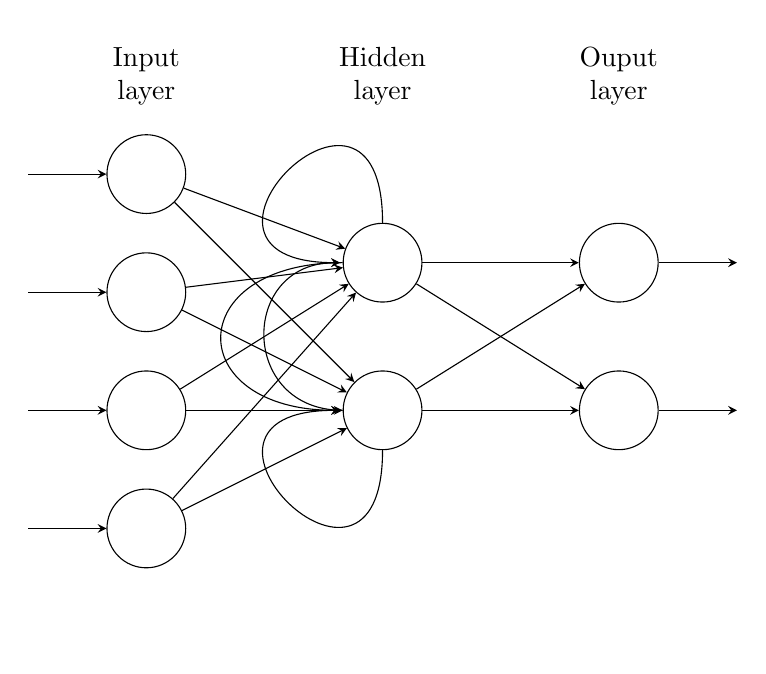
\begin{tikzpicture}[x=1.5cm, y=1.5cm, >=stealth]

\foreach \m/\l [count=\y] in {1,2,3,4}
  \node [every neuron/.try, neuron \m/.try] (input-\m) at (0,2.5-\y) {};

\foreach \m [count=\y] in {1,2}
  \node [every neuron/.try, neuron \m/.try ] (hidden-\m) at (2,2-\y*1.25) {};

\foreach \m [count=\y] in {1,2}
  \node [every neuron/.try, neuron \m/.try ] (output-\m) at (4,2-\y*1.25) {};

\foreach \l [count=\i] in {1,2,3,n}
  \draw [<-] (input-\i) -- ++(-1,0)
    node [above, midway] {};

\foreach \l [count=\i] in {1,n}
  \node [above] at (hidden-\i.north) {};

\foreach \l [count=\i] in {1,n}
  \draw [->] (output-\i) -- ++(1,0)
    node [above, midway] {};

\foreach \i in {1,...,4}
  \foreach \j in {1,...,2}
    \draw [->] (input-\i) -- (hidden-\j);

\foreach \i in {1,...,2}
  \foreach \j in {1,...,2}
    \draw [->] (hidden-\i) -- (output-\j);

\draw[->,shorten >=1pt] (hidden-1) to [out=90,in=180,loop,looseness=8.8] (hidden-1);
\draw[->,shorten >=1pt] (hidden-2) to [out=-90,in=180,loop,looseness=8.8] (hidden-2);

\draw[->,shorten >=1pt] (hidden-1) to [out=180,in=180,loop,looseness=2.8] (hidden-2);
\draw[->,shorten >=1pt] (hidden-2) to [out=180,in=180,loop,looseness=1.8] (hidden-1);


\foreach \l [count=\x from 0] in {Input, Hidden, Ouput}
  \node [align=center, above] at (\x*2,2) {\l \\ layer};

\end{tikzpicture}
\caption{Recurrent Neural Network}
\label{fig:RNN}
\end{center}
\end{figure}